\section{Algoritmos gen\'eticos}
%{\it Revisar informaci\'on de }\cite{Alex2005}{\it y modificar lo que
%se deba de esta secci\'on...} 
La construcci\'on de computadoras m\'as r\'apidas y econ\'omicas 
durante las \'ultimas d\'ecadas ha permitido que t\'ecnicas 
novedosas, las cuales demandan mucho de las computadoras, se vuelvan 
una alternativa realizable. Una de las \'areas m\'as prometedoras 
para llevar a cabo un r\'apido crecimiento es la computaci\'on 
evolutiva, particularmente los llamados algoritmos gen\'eticos (AG) 
\citep{Kur199901}.

Un AG es un procedimiento computacional el cual intenta caracterizar 
lo esencial de un sistema simulando parcialmente el proceso de 
selecci\'on natural, con la intenci\'on de resolver problemas de 
optimizaci\'on. La caracterizaci\'on de un sistema depende en gran 
medida del modelo adoptado. Mucho del arte de la computaci\'on 
evolutiva en general y en los algoritmos gen\'eticos en particular 
depende de la habilidad de reflejar en el modelo la naturaleza 
verdadera del sistema.

Los AG se implementan como una simulaci\'on por computadora en la que
una poblaci\'on, donde cada individuo es un conjunto de valores que 
representa un candidato a soluci\'on, evoluciona de tal manera que 
cada generaci\'on contiene individuos con mayor probabilidad de ser 
la mejor soluci\'on. La evoluci\'on sucede por generaciones y 
com\'unmente inicia a partir de una poblaci\'on de individuos 
generados aleatoriamente. 

Cada generaci\'on es una iteraci\'on de AG y en ella se eval\'ua la 
aptitud de cada individuo, se selecciona un conjunto y se modifica 
aplic\'andole operadores gen\'eticos para formar la poblaci\'on de la 
siguiente generaci\'on. Son tres los mecanismos b\'asicos (operadores 
gen\'eticos) que normalmente son considerados el origen del poder de
los AG: la selecci\'on, la reproducci\'on y la mutaci\'on 
\footnote{Para explicaci\'on m\'as extensa de AG ver 
\cite{Kur199901}.}.

\subsection{Selecci\'on}
%%\paragraph{Introducci\'on a la selecci\'on}
En cada generaci\'on se selecciona una porci\'on de la poblaci\'on 
existente para producir la nueva generaci\'on. La selecci\'on se basa
en la aptitud, donde las soluciones m\'as aptas tienen mayor 
probabilidad de ser seleccionadas. 

%\paragraph{Selecci\'on Estoc\'astica}
La mayor\'ia de los m\'etodos de selecci\'on son estoc\'asticos de 
tal manera que una peque\~na parte de las soluciones menos aptas 
tambi\'en son seleccionadas. Esto ayuda a mantener alta diversidad en
la poblaci\'on, evitando convergencias prematuras hacia m\'aximos o 
m\'inimos locales \citep{Kur199901}.

%\paragraph{Selecci\'on Utilizada}
La selecci\'on tambi\'en puede ser determinista, es decir, los 
descendientes son seleccionados de alguna forma espec\'ifica. En el 
presente trabajo la selecci\'on fue determinista y elitista: solo los
$n/4$ individuos m\'as aptos, con un valor en la funci\'on 
deseabilidad menor y donde $n$ es el tama\~no inicial de la 
poblaci\'on, tienen la oportunidad de reproducirse. 

\subsection{Reproducci\'on}
%\paragraph{Reproducci\'on y tama\~no de la poblaci\'on}
Para ir de una generaci\'on a otra hay dos estrategias b\'asicas: que
cada individuo d\'e origen a un nuevo individuo o d\'e origen a m\'as
de uno. En el primer caso el tama\~no de la poblaci\'on se mantiene 
constante, mientras que en la segunda opci\'on crece con el tiempo.

%\paragraph{Introducci\'on a la reproducci\'on}
Una vez que se hizo la selecci\'on de la poblaci\'on se decidi\'o 
hacer parejas de individuos ordenados seg\'un su aptitud con la 
intenci\'on de reproducirlos. Cada pareja genera 2 nuevos individuos.
Cada uno de los individuos est\'a formado por un conjunto de genes. 
Cada gen representa una posici\'on de una mol\'ecula de agua, por lo 
tanto el m\'aximo n\'umero de genes que se utilizan en este trabajo es
9, pues se est\'a interesado en investigar la hidrataci\'on con 9
mol\'eculas de agua en al primera capa de hidrataci\'on y ninguna en
la segunda u 8 en la primera y una en la segunda. Dos individuos 
pudieran ser 
\be\label{induno}
\left[\ba{ccccccccc}
\vec r_{1,1}&\vec r_{2,1} &\vec r_{3,1} &\vec r_{4,1} &\vec r_{5,1} 
&\vec r_{6,1} &\vec r_{7,1} &\vec r_{8,1} &\vec r_{9,1} 
\ea\right]
\ee
y
\be\label{inddos}
\left[\ba{ccccccccc}
\vec r_{1,2} &\vec r_{2,2} &\vec r_{3,2} &\vec r_{4,2} &\vec r_{5,2} 
&\vec r_{6,2} &\vec r_{7,2} &\vec r_{8,2} &\vec r_{9,2} 
\ea\right].
\ee
La combinaci\'on de genes en la reproducci\'on se determina de
manera aleatoria, por ejemplo un pap\'a pudiera ser ~(\ref{induno}) y
los genes que hereda al hijo ser los elementos de valor 1 en un 
vector, $P$, generado aleatoriamente, por ejemplo
\be\label{papa}
P=[1 0 0 1 0 1 1 0 0];
\ee
y la mam\'a pudiera ser ~(\ref{inddos}) y sus genes heredados ser\'an
los correspondientes a los elemento con valor 1 en un vector $M$ 
complemento de $P$
\be\label{mama}
M=[0 1 1 0 1 0 0 1 1],
\ee
entonces, un hijo ser\'ia
$$
\left[\ba{ccccccccccc}
\vec r_{1,1} &\vec r_{2,2} &\vec r_{3,2} &\vec r_{4,1} &\vec r_{5,2} 
&\vec r_{6,1} &\vec r_{7,1} &\vec r_{8,2} &\vec r_{9,2} &
\ea\right],
$$
y su mellizo ser\'ia la combinaci\'on de los genes de ~(\ref{inddos}) a
los que les corresponden un 1 en los elementos de ~(\ref{papa}) y los
genes de ~(\ref{induno}) correspondientes a los elementos con valor 1
en ~(\ref{mama})
$$
\left[\ba{ccccccccccc}
\vec r_{1,2} &\vec r_{2,1} &\vec r_{3,1} &\vec r_{4,2} &\vec r_{5,1} 
&\vec r_{6,2} &\vec r_{7,2} &\vec r_{8,1} &\vec r_{9,1} &
\ea\right].
$$

%\paragraph{Reproducci\'on Usada}
En las estrategias Vasconcelos y Nietzsche \citep{Kur199901} la 
selecci\'on de parejas de progenitores en la reproducci\'on es 
determinista. En el presente trabajo la selecci\'on es elitista: solo
los $n/4$ individuos m\'as aptos, donde $n=48$ es el tama\~no de la 
poblaci\'on inicial, tienen la posibilidad de reproducirse, y las 
parejas de individuos progenitores son hechas de una manera determinista, es 
decir, la elecci\'on de ~(\ref{induno}) y ~(\ref{inddos}) se hizo 
dependiendo de la aptitud de cada individuo. Aqu\'i se us\'o la 
estrategia Vasconcelos, es decir, el mejor individuo se cruza con el 
peor de los individuos, el segundo mejor con el segundo peor 
individuo, etc. Hasta este momento el tama\~no de la poblaci\'on es 
de $n/2$.

\subsection{Mutaci\'on}
%\paragraph{Introducci\'on a la mutaci\'on}
Los individuos de la nueva poblaci\'on son resultado de la 
recombinaci\'on gen\'etica. Se espera que los nuevos individuos 
tengan una mejor aptitud, pero los genes posibles no cambian. Para 
modificar esto, despu\'es del proceso de reproducci\'on se les 
permite la posibilidad de una peque\~na modificaci\'on en los genes
de cada uno de los $n/2$ individuos, generando otros $n/2$ individuos
con algunos genes diferentes a los contenidos en los primeros $n/2$
posibles soluciones existentes despu\'es de la reproducci\'on.

%\paragraph{}
En el presente trabajo las mutaciones corresponden a desplazamientos 
de las mol\'eculas de agua r\'igidas y deformaciones de las 
mol\'eculas. Se les permite un desplazamiento hasta de 0.03464 {\AA} 
en cada una de las direcciones y una deformaci\'on de las mol\'eculas
debido a desplazamientos de los \'atomos de hidr\'ogeno hasta de
0.001732 {\AA} en cada una coordenadas de cada hidr\'ogeno. A todas 
las mol\'eculas y \'atomos de hidr\'ogeno se les permite mutar.

\subsection{Evaluaci\'on de la aptitud}
Como lo que se quiere encontrar son los genes que puedan proporcionar
la estructura m\'as estable, la funci\'on deseabilidad que se 
utiliz\'o fue la energ\'ia de cada una de las configuraciones 
obtenidas a partir de c\'alculos {\it single point} utilizando el
software Gaussian 09. Los c\'alculos de las energ\'ias fueron 
realizadas utilizando PCM a un nivel MP2. 

%\ocultartrue 
%\begin{Vocultar}
%reproducir 
%los datos experimentales de la matriz de mezcla y la violaci\'on de 
%$CP$, se us\'o una funci\'on de deseabilidad compuesta por 12 
%funciones, una por cada dato experimental. Cada una de las 12 
%funciones son del tipo de Derringer \cite{rayon}, est\'an compuestas 
%por tres rectas (cuando en valor se $s=1$ como se explica a 
%continuaci\'on), una de pendiene cero y valor 1 para todo dato dentro
%del error experimental, al que se le referir\'a como intervalo 
%experimental,  y las otras dos con pendientes iguales pero de signo
%contrario. El valor m\'inimo de cada funci\'on individual es cero y 
%corresponde al valor en el dominio m\'as alejado de los valores 
%extremos del intervalo experimental y es 1 cuando se est\'a dentro de
%dicho intervalo.
%
%Por ejemplo, el dominio para cada m\'odulo de los nueve elementos de
%la matriz de mezcla es de cero a uno, $0\leq |V_{ij}|\leq 1$. Para 
%los tres m\'odulos de la diagonal el valor m\'as alejado de 
%cualquiera de los dos extremos del intervalo experimental es el cero,
%entonces, la funci\'on deseabilidad es
%\be\label{fund}
%d_i=\left\{\ba{ll} \left[\frac{|V_{ii}|}{VI_{ii}}\right]^s
%                   &0\leq |V_{ii}|\leq VI_{ii}\\
%                   \left[\frac{-|V_{ii}|}{VI_{ii}}+
%                   \frac{VI_{ii}+VS_{ii}}{VI_{ii}}\right]^s
%                    &VS_{ii}\leq |V_{ii}|\leq 1\\
%                    1&VI_{ii}\leq|V_{ii}|\leq VS_{ii}\ea\right .
%\ee   
%donde $VI_{ii}$ es el valor inferior del intervalo experimental para 
%el m\'odulo de la matriz de mezcla, $VS_{ii}$ es el valor superior 
%del intervalo, $|V_{ii}|$ es el valor obtenido del modelo y $s$ es el
%exponencial propuesto por Derringer con el objetivo de que $d_i$ tome
%valores grandes solo cuando est\'e cerca de entrar al intervalo 
%experimental. Para los m\'odulos de la matriz de mezcla, en el 
%presente trabajo, el exponente $s$ se eligi\'o con el valor $s=5$. 
%Para el invariante de Jarlskog y los \'angulos $\alpha$ y $\gamma$ 
%del tri\'angulo unitario los dominios son $-1\leq J\leq 1$ y 
%$0\leq \mbox{\'angulo}\leq360$ respectivamente y sus funciones 
%deseabilidad ($d_J$, $d_{\alpha}$ y  $d_{\gamma}$) son de la misma 
%forma a la ecuaci\'on ~\ref{fund}, sus respectivas $s$ son 15 y 10. 
%Para los otros seis m\'odulos el valor m\'as alejado de los extremos 
%de los intervalos experimentales es 1 y las funciones deseabilidad
%tienen la forma  
%\be\label{fund1}
%d_i=\left\{\ba{ll} \left[\frac{|V_{ij}|}{VS_{ij}}+
%                   \frac{1-VS_{ij}-VI{ij}}{1-VS_{ij}}\right]^s
%                   &0\leq |V_{ij}|\leq VI_{ij}\\
%                   \left[\frac{-|V_{ij}|}{1-VS_{ij}}+
%                   \frac{1}{1-VS_{ij}}\right]^s
%                    &VS_{ij}\leq |V_{ij}|\leq 1\\
%                    1&VI_{ij}\leq|V_{ij}|\leq VS_{ij}\ea\right .
%\ee   
%%%%%%%%%%%%%%%%%%%%%%%%%%%%%%%%%%%%%%%%%%%%%%%%%%%5555
%\begin{figure}\label{fig1}
%\centering
%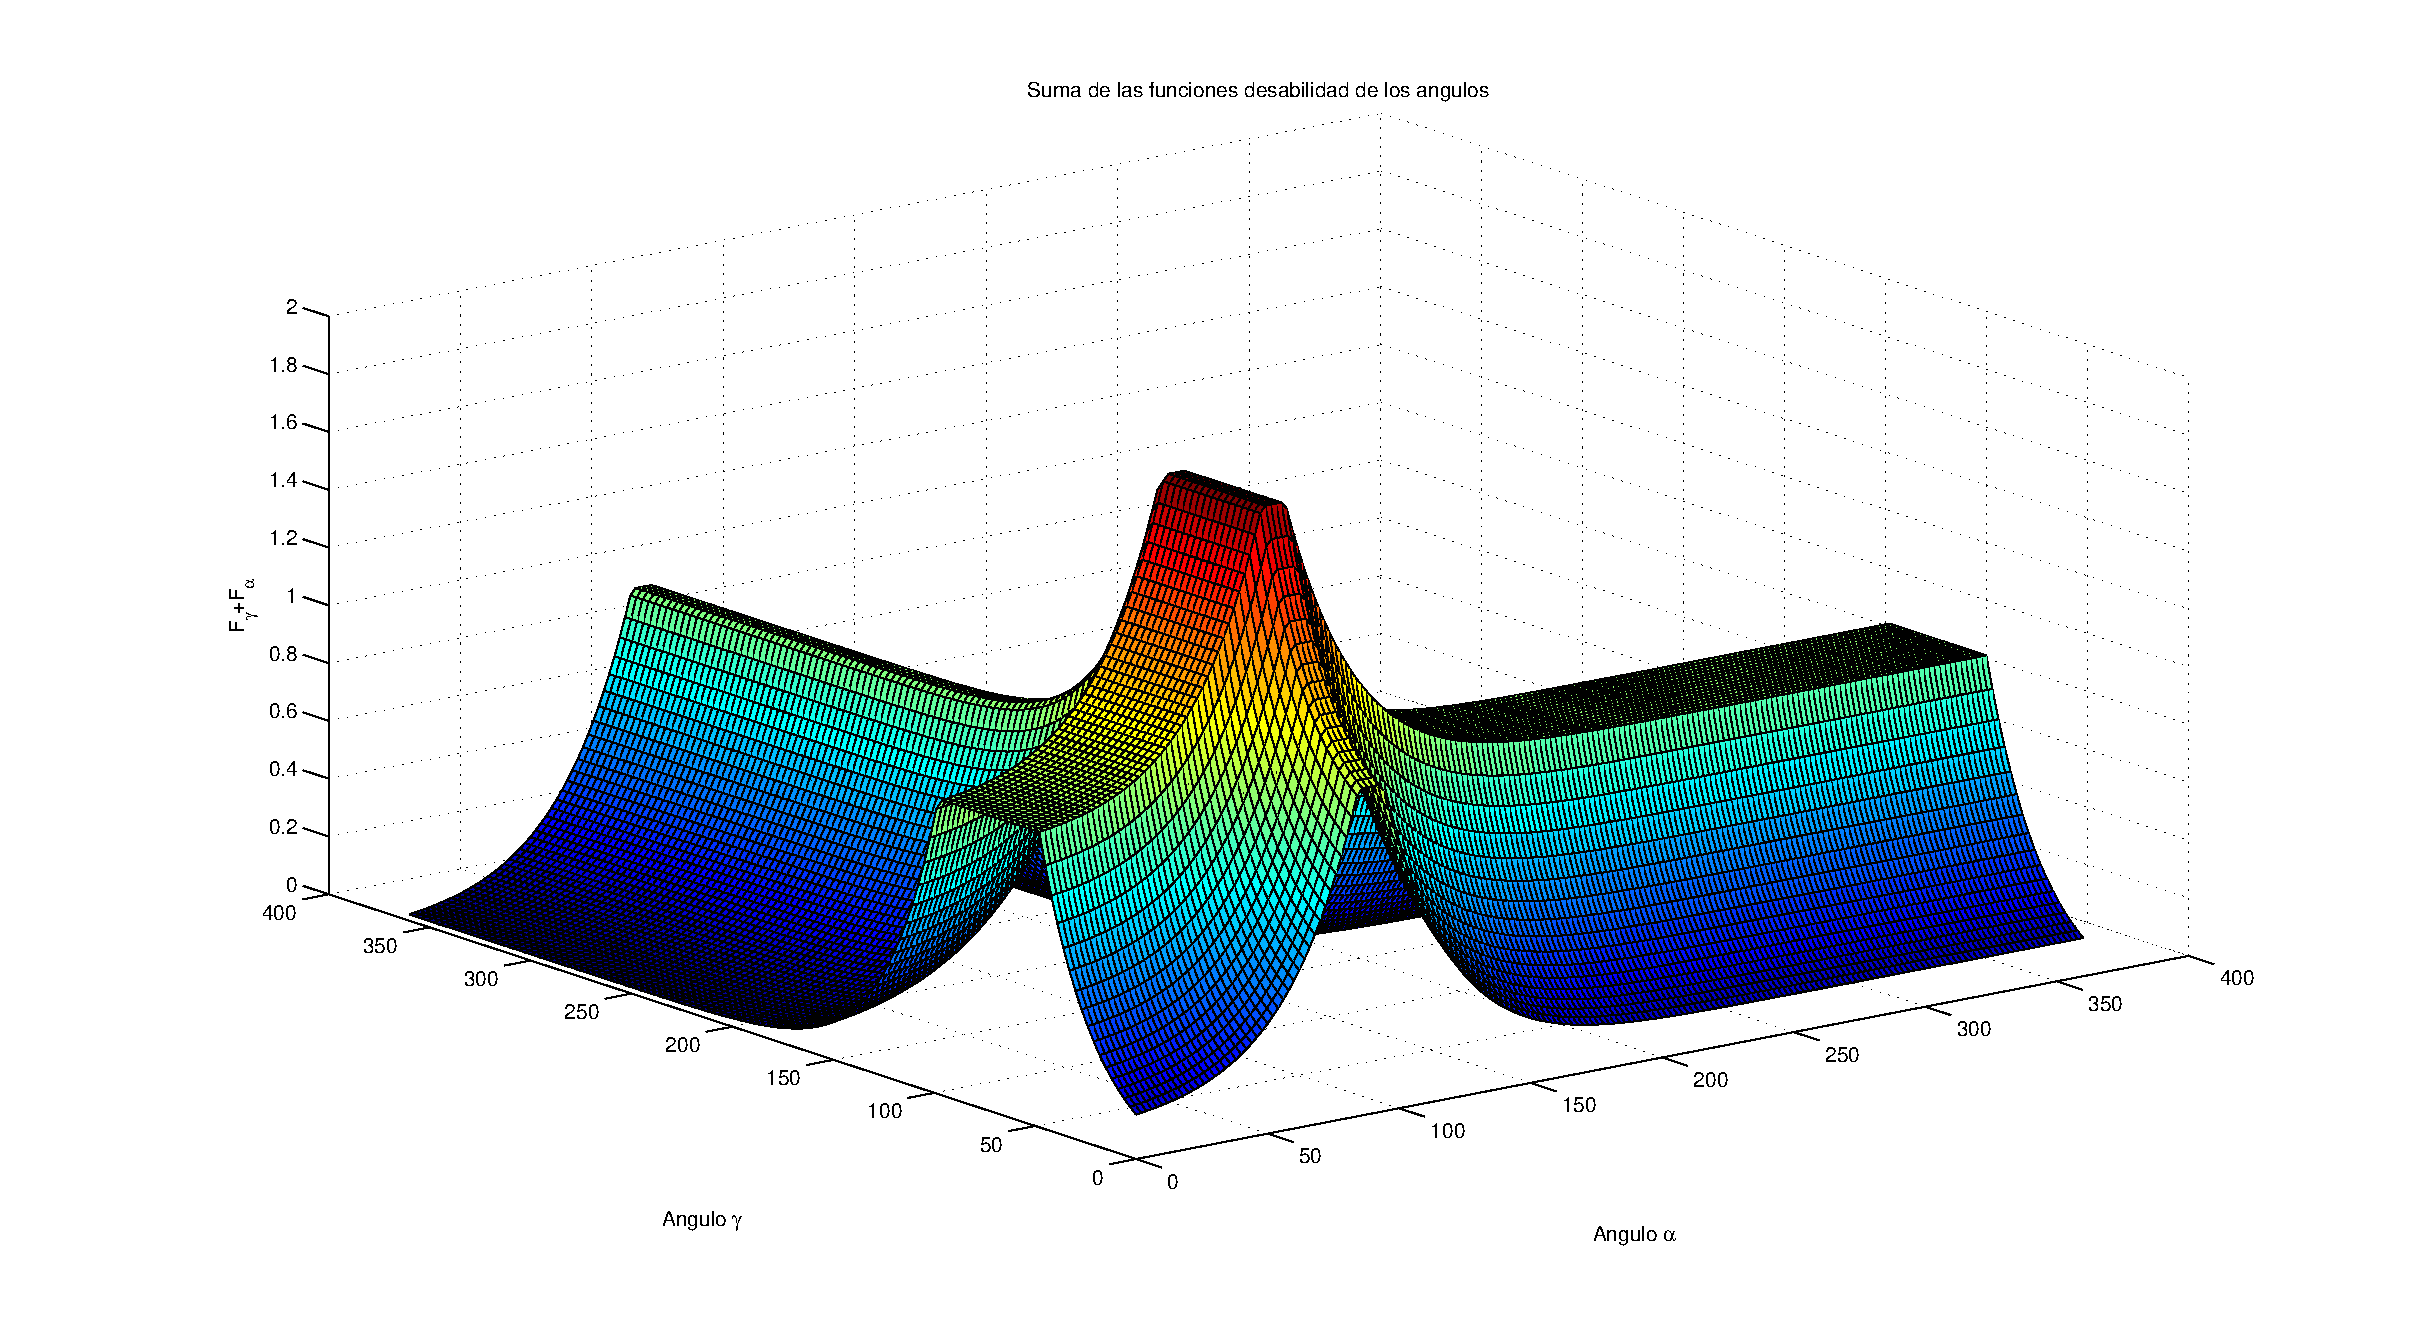
\includegraphics[height=9cm,angle=0]{../Tesis/Graficas/fdeseabilidadsuma.eps}
%\caption{Suma de las funciones deseabilidad tipo Derringer de los \'angulos 
%internos del tri\'angulo unitario}
%\end{figure}
%%%%%%%%%%%%%%%%%%%%%%%%%%%%%%%%%%%%%%%%%%%%%%%%%%%%%%%
%La suma de las funciones deseabilidad para los dos \'angulos ($d_{\alpha}$ y 
%$d_{\gamma}$) calculados por el AG se muestra en la figura 3.2.
%%~\ref{fig1}.
%
%
%Para encontrar las matrices de masa de los quarks compatibles con los datos 
%experimentales se utliza AG para optimizar la funci\'on  deseabilidad, $F_d$,
%que es la suma de las doce funciones individuales
%$$F_d=\sum^{12}_{i=1}d_i+d_J+d_{\alpha}+d_{\gamma},$$
%y tiene un valor m\'aximo de 12, justo cuando los doce par\'ametros que se
%intentan ajustar est\'an dentro del intervalo experimental.  
%\end{Vocultar}

\subsection{Validaci\'on del AG}
%\paragraph{?`C\'omo se valid\'o el AG?}
Aqu\'i debo de agregar el c\'omo.
